\documentclass[onecolumn, draftclsnofoot,10pt, compsoc]{IEEEtran}
\usepackage{graphicx}
\usepackage{url}
\usepackage{setspace}
\usepackage{array}
\usepackage{advdate}
\usepackage{caption}

\usepackage{geometry}
\geometry{textheight=9.5in, textwidth=7in}

% 1. Fill in these details
\def \CapstoneTeamName{Proprietors of the Press}
\def \CapstoneTeamNumber{62}
\def \GroupMemberOne{Kuan-Yu Lai}
\def \GroupMemberTwo{Cole Jones}
\def \CapstoneProjectName{Automate the Settings that Control a Million-Dollar Printing Press}
\def \CapstoneSponsorCompany{HP, Inc}
\def \CapstoneSponsorPersonA{Pieter van Zee}
\def \CapstoneSponsorPersonB{Ronald Tippetts}

% 2. Uncomment the appropriate line below so that the document type works
\def \DocType{Winter Term Final Progress Report}
			
\newcommand{\NameSigPair}[1]{\par
\makebox[2.75in][r]{#1} \hfil 	\makebox[3.25in]{\makebox[2.25in]{\hrulefill} \hfill		\makebox[.75in]{\hrulefill}}
\par\vspace{-12pt} \textit{\tiny\noindent
\makebox[2.75in]{} \hfil		\makebox[3.25in]{\makebox[2.25in][r]{Signature} \hfill	\makebox[.75in][r]{Date}}}}
% 3. If the document is not to be signed, uncomment the RENEWcommand below
\renewcommand{\NameSigPair}[1]{#1}

%%%%%%%%%%%%%%%%%%%%%%%%%%%%%%%%%%%%%%%
\begin{document}
\begin{titlepage}
    \pagenumbering{gobble}
    \begin{singlespace}
    	%\includegraphics[height=4cm]{coe_v_spot1}
        \hfill 
        % 4. If you have a logo, use this includegraphics command to put it on the coversheet.
        %\includegraphics[height=4cm]{CompanyLogo}   
        \par\vspace{.2in}
        \centering
        \scshape{
            \huge CS Capstone \DocType \par
            {\large\AdvanceDate[-1]\today}\par
            \vspace{1.0in}
            \textbf{\Huge\CapstoneProjectName}\par
            \vfill
            {\large Prepared for}\par
            \Huge \CapstoneSponsorCompany\par
            \vspace{5pt}
            {\Large\NameSigPair{\CapstoneSponsorPersonA}\par}
            {\Large\NameSigPair{\CapstoneSponsorPersonB}\par}
            {\large Prepared by }\par
            Group\CapstoneTeamNumber\par
            % 5. comment out the line below this one if you do not wish to name your team
            \CapstoneTeamName\par 
            \vspace{5pt}
            {\Large
                \NameSigPair{\GroupMemberOne}\par
                \NameSigPair{\GroupMemberTwo}\par
            }
            \vspace{20pt}
        }
        \vspace{72pt}
        \begin{abstract}
            % 6. Fill in your abstract    
        	This document describes the project in its current state. It outlines where we are currently at in the project's development, some difficulties that were encountered in its implementation, work that is still remaining before the project's full release, and code that we found particularly interesting. Also, some pictures are supplied of the project's front-end in its current state.
        \end{abstract}
    \end{singlespace}
\end{titlepage}
\newpage
\pagenumbering{arabic}
% 7. uncomment this (if applicable). Consider adding a page break.
\tableofcontents
\listoffigures
%\listoftables
\clearpage

% Set single spacing
\singlespacing

% 8. now you write!
\section{Project Recap}
The purpose of this project is to simplify the process of choosing the correct press settings for a given print job. Print job settings will be determined through the use of a Rules Engine, which will take a collection of user inputs about a job (i.e. the type of paper, the selected press, the maximum ink coverage, etc.) and apply them to a set of rules (which may be different for each press). The output of the Rules Engine will be the optimal press settings for the given print job.\\[10pt]
The goal of this project is to simplify the settings selection process so that any employee may generate press settings, not just specially-trained ones. Users will fill out a form on a website front-end to provide some information about the print job, and the Rules Engine will do the rest of the work.

\vspace*{\floatsep}
\section{Current Progress}
\subsection{Front-End}
The website in its current form has three pages (other than the home page): the New Job page; the Job Results page, which is only accessed from the New Job page upon submitting the form; the Job History page.

% Main page of the website
\begin{figure}[!ht]
    \makebox[\textwidth][c]{
\includegraphics[width=1.0\textwidth]{Images/HomePage.PNG}}
    \caption{The home page of the website}
    \label{fig:1}
\end{figure}

\noindent The New Job page (fig. 2) provides a form to the user where they are able to enter information about the print job, such as the job's name, quality mode, max coverage, optical density, and which paper it will be printed on. When the user clicks the 'Submit' button on the form, all of the form data is sent to the Rules Engine where it will be processed. That POST call returns a Job ID, which is then used in the Job Results page (which the user is redirected to upon clicking submit).\\[10pt]
The Job Results page uses the passed Job ID to get the results of the Rules Engine from the file system (once the Rules Engine is done processing the job). The data in the job result is displayed to the user in a selectable spreadsheet for ease of copying data into Excel. In addition to the spreadsheet, there is an 'Export to CSV' button, which dumps the contents of the spreadsheet into a CSV file named after the job ID.\\[10pt]
The Job History page (fig. 3) is similar to the Job Results page, but it instead has a table of all previously-run jobs. The user is able to select a single job and display its results in a popup modal, or select multiple jobs and do a comparison between them (view them side-by-side). Within each modal, there is also an 'Export to CSV' button like the one on the Job Results page.

\newpage
\begin{figure}[!ht]
    % New Job page
    \makebox[\textwidth][c]{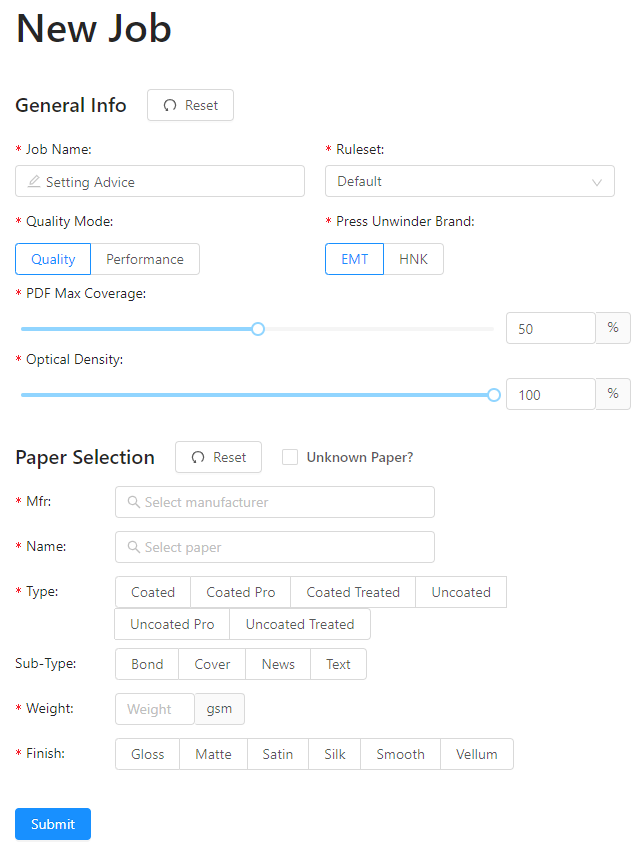
\includegraphics[width=0.55\textwidth]{Images/NewJob.PNG}}
    \caption{The New Job form}
    \label{fig:2}
    \vspace*{\floatsep}
    % Job History Page
    \makebox[\textwidth][c]{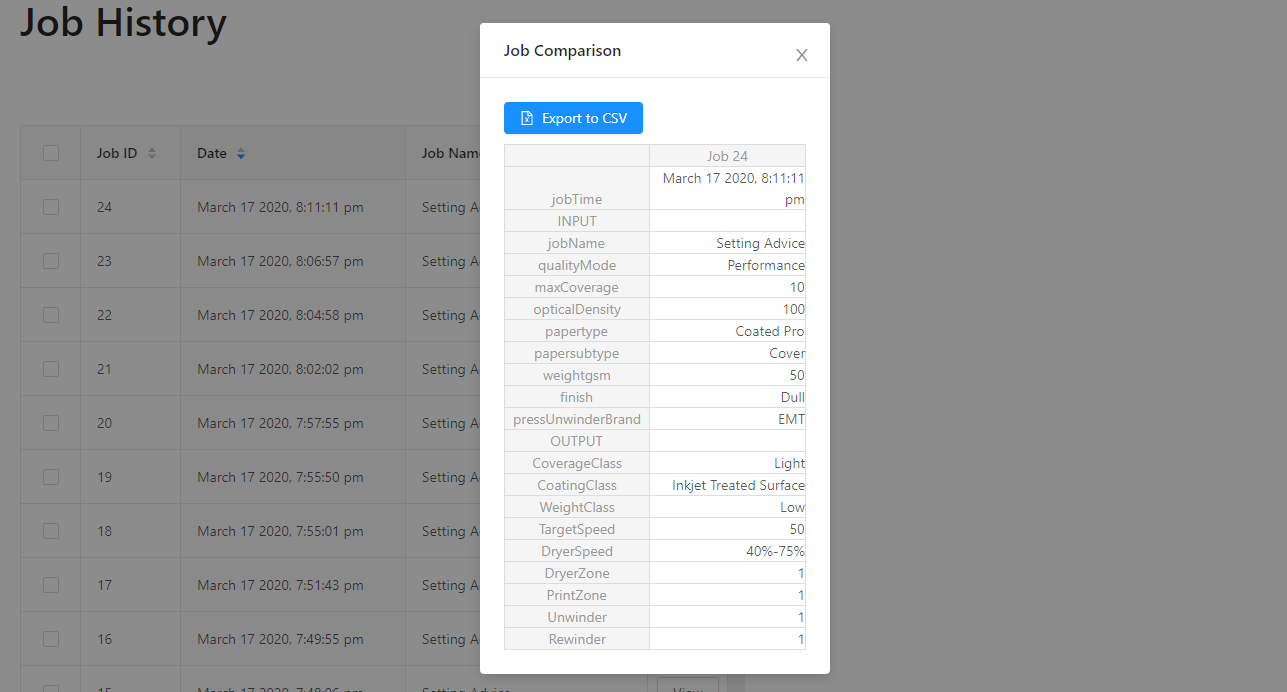
\includegraphics[width=0.8\textwidth]{Images/JobHistory.PNG}}
    \caption{The Job History page}
    \label{fig:3}
\end{figure}

\newpage
\subsection{Back-End}
The back-end now has two servers that host two different engines: the SJA Engine and the Rules Engine. Both of the servers are hosted on AWS, but with different EC2 servers. The SJA Engine is the engine that controls all the flows in the back-end. It is also a RESTful API that interacts with the front-end website and the file system of the application. Once the SJA Engine gets the data back from the Rules Engine, it will document the detailed information in a JSON file. It can either send all records or a specific record based on the given ID to the front-end.\\[10pt]
The Rules Engine is the engine that generates the recommended settings based on the given settings. It evaluates the settings by using the rule files of the selected ruleset. The rule files are pre-defined and can easily be changed by the developer. The constrains inside those rule files is defined by the expert from HP. 

\vspace*{\floatsep}
\section{Remaining Work}
\subsection{Front-End}
Our client wants some additional functionality to be added to the spreadsheet in Job Results and Job History. They want an additional column added to hold the justifications that the Rules Engine will eventually supply, and they want it to be toggle-able so that they can choose whether or not it will be included in the CSV export.\\[10pt]
They also want additional columns in the table in Job History, so that additional information about the job can be displayed without having to actually view the results.\\[10pt]
Finally, they want browser cookies to remember previous selections on the New Job page for things that rarely change, such as quality mode and press unwinder brand, so that a user does not have to change them every time.

\subsection{Back-End} 
The remaining work of the back-end will be to improve the accuracy of the Rules Engine and implement the justifications. Ideally, the Rules Engine will be able to process the settings for all the different printing presses that HP has. So we still have to create more rule files and implement more constraints inside those files. Also, we have to create different rulesets to handle different situations from the user, and decide which rule files different rulesets should contain.\\[10pt]
For the supply justification feature, it's the feature that provides the different reasons why the Rules Engine decides each setting. So basically, provide the constraints that the Rules Engine used and translate that to the user-readable words.

\vspace*{\floatsep}
\section{Problems}
\subsection{Front-End}
There was a fairly big struggle getting the fetch calls to the back-end's endpoints to work properly. Because the endpoint was using http and the rendered website was using https, Google Chrome was throwing a 'Mixed Content' error and preventing the call from executing. A significant amount of time was spent debugging the error because it was so cryptic. In the end, it was found that appending a 'cors' tag to the POST/GET call bypassed the error, allowing the site to use the endpoints properly.\\[10pt]
Recently, Ant Design, the UI framework that we're using, had a major update from version 3.X to version 4.X. This caused a lot of the documentation to change to suit the new version. This was a source of some confusion, as the change was not immediately noticed. An attempts was made to port the existing site to version 4.X, but it was found that some of the new implementations for the components we're using were significantly different. In the end, we decided to stick with version 3.X, since it has not been depreciated and is still valid.\\[10pt]
There was an issue for a while where some components were causing the state to update very rapidly, which in turn caused the normally fast and responsive components to cause a fair bit of lag. It took many hours to figure out how to prevent these unnecessary state updates, but in the end a solution was found. Some of the logic was changed to add debouncing, so that the component would not update the state until there were no changes in its data for a small amount of time.

\subsection{Back-End}
At the beginning of the term, we were testing two different Rules Engines, Drools and J-easy Rules. After several days of testing, we found that J-easy Rules was a better choice than Drools, because J-easy Rules is easier to be integrated with our program and the can support the needs of our project as well. Also, we both agree that j-easy is easier to learn and implement.\\[10pt]
Initially, we were developing our SJA Engine server with Python. But our client wants us to do develop all of the servers with Java-related language, for long term consideration. As a result, we chose JavaScript as our language to develop the SJA Engine and Java for the J-easy Rules Engine. The reason why we used Java to develop J-easy Rules Engine is that the library is coded in Java. \\[10pt]
The rules standard sent from our client is sometimes difficult to implement in the program. As a result, we often need to hard-code the rules instead of using the relation. This reduces the expandability of the program. In addition, we still have to discuss with our client to determine the belonging of each rule. 

\vspace*{\floatsep}
\section{Interesting Code}
\subsection{Front-End}
% Front-end code - narrow paper picklist on manufacturer select
\begin{figure}[!ht]
    \makebox[\textwidth][c]{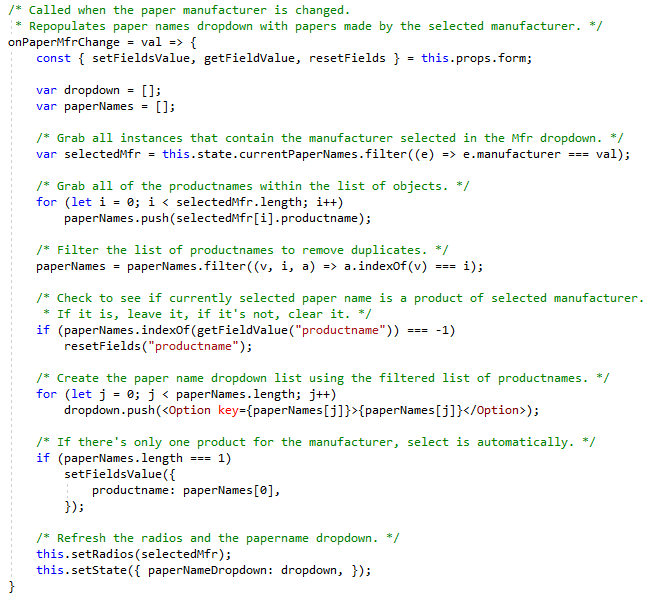
\includegraphics[width=0.75\textwidth]{Images/front_Code_1.PNG}}
    \caption{Paper list change upon selection of manufacturer}
    \label{fig:4}
\end{figure}
\noindent This code is interesting because of how long it took to implement. It took a good number of hours to figure out the logic to filter the list of available paper brands, as well as other options (type, finish, etc.), when a manufacturer was selected. Although it might not look so interesting visually, it is a proud achievement because of how much effort it took.

\newpage
\subsection{Back-End}
% Back-end code - yml file
\begin{figure}[!ht]
    \makebox[\textwidth][c]{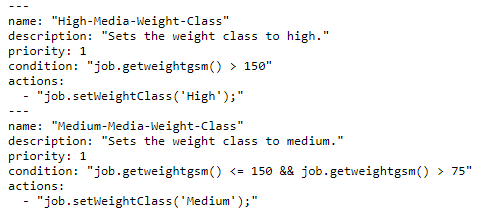
\includegraphics[width=0.7\textwidth]{Images/back_Code_1.PNG}}
    \caption{Rules definition in Rules Engine}
    \label{fig:5}
\end{figure}
\noindent This code is interesting because it provides to the developer the ability to change the constraints easily without recompiling the code. Also, developers can be able to make any constraints based on the given function inside the job class. 
\end{document}